\documentclass[amsmath,amssymb,floatfix]{revtex4}
%twocolumn
\usepackage{graphicx}% Include figure files
\usepackage{dcolumn}% Align table columns on decimal point
\usepackage{bm}% bold math
\usepackage{amssymb}
\usepackage{amsmath}
\usepackage{amsfonts}
\usepackage{epsf}
\usepackage{color} % allows color in fonts
\usepackage{verbatim}
\usepackage{listings}
\usepackage{xcolor}
\usepackage{titlesec}
\usepackage{float}
\usepackage{natbib}
\usepackage{subfigure}

\usepackage[brazilian]{babel}
\usepackage[utf8]{inputenc}
\usepackage[T1]{fontenc}

\newcommand{\PAR}[1]{\left({[#1]}\right)}
\newtheorem{defi}{Definição}[section]


\lstdefinestyle{customc}{
  belowcaptionskip=1\baselineskip,
  breaklines=true,
  frame=none,
  xleftmargin=\parindent,
  language=C,
  showstringspaces=false,
  basicstyle=\footnotesize\ttfamily,
  keywordstyle=\bfseries\color{green!40!black},
  commentstyle=\itshape\color{purple!40!black},
  identifierstyle=\color{blue},
  stringstyle=\color{orange},
}

\lstdefinestyle{customasm}{
  belowcaptionskip=1\baselineskip,
  frame=trBL,
  xleftmargin=\parindent,
  language=[x86masm]Assembler,
  basicstyle=\footnotesize\ttfamily,
  commentstyle=\itshape\color{purple!40!black},
}

\lstset{escapechar=@,style=customc}

\titlespacing\section{0pt}{12pt plus 4pt minus 2pt}{8pt plus 2pt minus 2pt}
\titlespacing\subsection{0pt}{12pt plus 4pt minus 2pt}{8pt plus 2pt minus 2pt}
\titlespacing\subsubsection{0pt}{12pt plus 4pt minus 2pt}{0pt plus 2pt minus 2pt}

%%%%%%%%%%%%%%%%%%%%%
\graphicspath{ {pic/} }
%%%%%%%%%%%%%%%%%%%%%
\begin{document}

%%%%%%%%%%%%%%%%%%%%%%
%%%%%%%%%%%%%%%%%%%%%%
% T I T U L O
%%%%%%%%%%%%%%%%%%%%%%
%%%%%%%%%%%%%%%%%%%%%%

\title{Métodos de passo simples para sistema de equações diferenciais ordinárias}

\author{Li M.N \\\small email@email.com.br} 
\affiliation{
Universidade ....\\
}

\begin{abstract}
\baselineskip 11pt
Neste trabalho apresentamos três métodos de passo simples para obtermos soluções aproximadas para um sistema de equações diferenciais ordinárias. Será abordado o método de Euler explícito, implícito e aprimorado onde apresentamos resultados que comprovam convergência dos métodos.
\end{abstract}

\maketitle

%%%%%%%%%%%%%%%%%%%%%%
%%%%%%%%%%%%%%%%%%%%%%
\section{Introdução e Conceitos}
%%%%%%%%%%%%%%%%%%%%%%
%%%%%%%%%%%%%%%%%%%%%%

Modelagem é o processo em que um problema real seja ele físico, químico, biológico entre outros é traduzido em um modelo matemático envolvendo algum tipo de equação diferencial ou um sistema de equações diferenciais. No entanto, grande parte dos problemas matemáticos que envolvem problemas práticos, não possui solução analítica (exata) ou esta não é de fácil resolução. Isso ocorre devido às não-linearidades inerentes ao próprio comportamento do processo a ser analisado \cite{sebastiao}.
Por conta disso, é necessário utilizarmos de métodos que nos forneçam soluções aproximadas para a solução analítica do problema, são os chamados métodos numéricos.

Neste trabalho analisaremos alguns métodos de passo simples na solução de um problema de valor inicial envolvendo um sistema de equações diferenciais ordinárias dado em \eqref{sistemaPC}. Antes de prosseguirmos, é importante ressaltar que o desenvolvimento dos métodos numéricos pressupõe resultados teóricos envolvendo as equações diferenciais ordinárias, como existência e unicidade da solução e dependência contínua da solução com relação aos parâmetros e das condições iniciais. Pelo fato de conhecermos exatamente a solução do problema, equação \eqref{sol_exata}, esta satisfazer o sistema \eqref{sistemaPC}, não demonstraremos tais resultados teóricos. %No entanto, se o leitor achar necessário poderá consultar em qualquer livro .  %arrumar esse final do leitor  

Vamos utilizar um sistema de equações lineares com coeficientes variando no tempo dado por
\begin{equation}\label{sistemaPC}
\begin{cases}
\dot x=y  \qquad \qquad \qquad x(\sqrt{\pi}) = 0 \\
\dot y=y/t - 4t^2x \qquad y(\sqrt{\pi}) = -2\sqrt{\pi}
\end{cases}
\end{equation}
e que tem uma solução conhecida escrita como 
\begin{equation}\label{sol_exata}
\begin{cases}
 x(t)= \sin(t^2) \\ 
 y(t)= 2t\cos(t^2)
\end{cases}
\end{equation}

Neste artigo vamos implementar o método de Euler explícito, aprimorado e implícito para o sistema de equações \eqref{sistemaPC} a fim de obtermos soluções aproximadas. Para isso, dividimos o trabalho da seguinte maneira: na seção II apresentaremos o problema na forma normal de Cauchy além de sua discretização. Na seção III faremos uma breve introdução acerca dos métodos de passo simples e mostraremos os métodos que serão analisados neste trabalho. A próxima seção traz a implementação e o algoritmo utilizado para os métodos. A seção V aborda os métodos em si e seus resultados. E por fim, a última seção é a conclusão do trabalho.  

\section{Problema de Cauchy e discretização}
Vamos apresentar algumas definições que serão necessárias para o entendimento deste trabalho. 

\begin{defi}
Um problema de valor inicial ou problema de Cauchy é uma única equação ou um sistema de $m$ equações diferenciais ordinárias de primeira ordem, com $m$ condições iniciais conforme
\begin{equation}\label{formaPC}
\begin{cases}
\dot{y}(t)= f(t,y(t)), \qquad t \in [a,b], \\ 
 y(t_0)= y(a) = y_0.
\end{cases}
\end{equation}
\end{defi}  
A partir de um Problema de Cauchy para o qual as hipóteses de existência, unicidade e dependência contínua dos parâmetros e condição inicial com relação a solução estão satisfeitas, ver \cite{numerical}, podemos construir um problema de Cauchy aproximado. Ou seja, discretizamos o problema original \eqref{formaPC} e a solução é obtida para este novo problema, a solução numérica. Assim, a solução numérica só fica determinada em um conjunto discreto e finito de pontos conforme
\begin{equation*}
\begin{cases}
a=t_0, \\
t_1 = t_0 +\Delta t_1, \\
\vdots \\
b = t_n=t_{n-1} +\Delta t_n
\end{cases}
\end{equation*}
onde $\Delta t_1 = \Delta t_2 = \cdots = \Delta t_n = h = \frac{b-a}{n}$ é conhecido como passo de integração e n é o número de subintervalos de mesmo tamanho em $[a, b]$.

Para o problema \eqref{sistemaPC} podemos reescrevê-lo na forma normal de \eqref{formaPC} como segue
\begin{eqnarray*}
\dot{\mathbb{Y}}(t)
  = \begin{pmatrix} \dot x(t) \\ \dot y(t) \end{pmatrix}
  = \mathbb{F}(t, \mathbb{Y})
  = \begin{pmatrix} f_1(t,x(t),y(t))\\ f_2(t,x(t),y(t))\end{pmatrix}
 \end{eqnarray*}
 onde
 \begin{eqnarray}\label{nossoPC}
 \dot{\mathbb{Y}}(t)
  = \begin{pmatrix} \dot x(t) \\ \dot y(t) \end{pmatrix}
  = \mathbb{F}(t, \mathbb{Y})
 = \begin{pmatrix} y\\ y/t - 4t^2x \end{pmatrix}
 \end{eqnarray}
 e condições iniciais
 \begin{eqnarray}\label{nossaCI}
 {\mathbb{Y}_0}(t)
 =\begin{pmatrix}  x_0 \\ y_0 \end{pmatrix}
  = \begin{pmatrix}  x(\sqrt{\pi}) \\  y(\sqrt{\pi}) \end{pmatrix}
  = \begin{pmatrix} 0 \\ -2\sqrt{\pi} \end{pmatrix}
 \end{eqnarray}

\section{Métodos de passo simples}
Os métodos de passo simples ou também conhecidos como métodos de um passo são construídos a partir de combinações de polinômios de Taylor \cite{numerical,collatz} %numerical, kreysig.
Eles são da seguinte forma
\begin{equation}\label{def metodos}
\begin{cases}
 y_0 = y(t_0) \\ 
 y_{k+1} = y_k + h \Phi(t_k, t_{k+1}, y_k, y_{k+1}, h),
\end{cases}
\end{equation}
onde $\Phi(t_k, t_{k+1}, y_k, y_{k+1}, h)$ é chamada de função de discretização, $t_{k+1} = t_k + h$, com $0\leqslant k \leqslant n-1$ e $h = \frac{b-a}{n}$

Para diferenciarmos um método de passo simples explícito do implícito, devemos analisar a função de discretização $\Phi$. Se esta depender apenas de $(t_k,y_k,h)$, ou seja, nenhuma informação do instante posterior $t_{k+1}$ ele é denominado \textit{explícito}. Caso contrário, no \textit{implícito}, a $\Phi$ depende do valor de $y_{k+1}$ que está sendo calculada em $t_{k+1}$. Ou seja, temos que resolver uma equação algébrica em cada passo de integração para determinarmos a aproximação $y_{k+1}$. 

Assim, para o método de Euler explícito temos
\begin{equation}\label{def explicito}
\begin{cases}
 y_0 = y(t_0) \\ 
 y_{k+1} = y_k + h \Phi(t_k, y_k, h),
\end{cases}
\end{equation}
com $\Phi(t_k,y_k,h) \doteq f(t_k,y_k)$. No método de Euler implícito devemos ter
\begin{equation}\label{def implicito}
\begin{cases}
 y_0 = y(t_0) \\ 
 y_{k+1} = y_k + h \Phi(t_k, y_{k+1}, h),
\end{cases}
\end{equation}
com $\Phi(t_k,y_{k+1},h) \doteq f(t_k +h,y_{k+1})$. Observe que a aproximação $y_{k+1}$ possui $\Phi$ que também envolve o cálculo de $y_{k+1}$. É por isso que este método se chama implícito. Para o método de Euler aprimorado vamos ter
\begin{equation}\label{def aprimorado}
\begin{cases}
 y_0 = y(t_0) \\ 
 y_{k+1} = y_k + h \Phi(t_k, y_k, h),
\end{cases}
\end{equation}
com $\Phi(t_k,y_k,h) = \frac{1}{2} (\kappa_1 + \kappa_2)$ e 
\begin{equation*}
\begin{cases}
 \kappa_1 = f(t_k,y_k) \\ 
 \kappa_2 = f(t_k +h, y_k + h\kappa_1),
\end{cases}
\end{equation*} 

\section{Implementação e algoritmo}
O algoritmo foi implementado na linguagem Python, em três arquivo denominados \textit{EulerExplicito.py}, \textit{EulerAprimorado.py} e \textit{EulerImplicito.py}. Os gráficos foram gerados usando a biblioteca \textit{matplotlib} do Python.

Quando um dos arquivos \textit{.py} for rodado irá aparecer um menu de opções com 8 opções. São elas:
\begin{itemize}
\item[1.] Gráfico $x$ vs $t$ - diferentes $n$.
\item[2.] Gráfico $y$ vs $t$ - diferentes $n$.
\item[3.] Gráfico $x$ vs $t$ - solução exata e numérica.
\item[4.] Gráfico $y$ vs $t$ - solução exata e numérica.
\item[5.] Gráfico $x,y$ vs $t$ - solução exata e numérica.
\item[6.] Tabela erro de discretização COM solução exata.
\item[7.] Tabela erro de discretização SEM solução exata.
\item[8.] Sair do teste.
\end{itemize}

O usuário deverá escolher dentre as opções apresentadas. Se o arquivo \textit{EulerExplicito.py} for executado, cada uma das opções acima apresentarão os gráficos e tabelas que constam na seção do Método de Euler Explícito. O mesmo ocorre quando os arquivos \textit{EulerAprimorado.py} e \textit{EulerImplicito.py} foram executados. Para sair do teste basta escolher a opção $8$ e a execução do arquivo será finalizada.   

As funções específicas criadas para a execução de cada método serão apresentadas na sua subseção correspondente. Algumas funções gerais utilizadas nos três métodos segue abaixo:
\begin{lstlisting}
// condicoes iniciais
// t=np.sqrt(np.pi)
// xin=0
// yin=-2*(np.sqrt(np.pi))
// tfin=np.sqrt(4*np.pi)

// define a funcao (f1  e f2 da tarefa)
def F(t,y_i):
  f1 = y_i[1]
  f2 = (y_i[1])/t -4*(y_i[0])*(t**2)
  return np.array([f1,f2])

// define a funcao de discretizacao phi
def Phi(F,t,y_i,dt):
    p1 = F(t,y_i) // funcao phi para metodo de euler (kappa_1)
    p2 = F(t+dt, y_i + dt*p1) //funcao phi para metodo de euler aprimorado (kappa_2) 
    return np.array([p1,p2])
\end{lstlisting}
 
\section{Testes}
Nesta seção iremos apresentar os métodos utilizados no problema \eqref{nossoPC}-\eqref{nossaCI} com os códigos implementados em cada método e seus resultados. 

\subsection{Método de Euler Explícito}\label{sec:explicito}
Para determinarmos aproximações para a solução do problema \eqref{nossoPC}-\eqref{nossaCI}, devemos primeiramente discretizar o domínio de definição do problema. Como não foi imposto o valor para $b = t_n$, vamos utilizar $t_n = 2\sqrt{\pi}$. Assim, o intervalo $[\sqrt{\pi}, 2\sqrt{\pi}] \in$ \textit{Dom}$(\mathbb{Y}(t))$ e $n \in \mathbb{N}$ definido por $h = \Delta t = \frac{t_n - t_0}{n}$ é o número de passos de integração.

A discretização do problema \eqref{nossoPC} segundo o método dado por \eqref{def explicito} fornece 
\begin{eqnarray}\label{Explicito}
\begin{pmatrix}  x_{k+1} \\ y_{k+1} \end{pmatrix}
 = \begin{pmatrix} x_k\\ y_k \end{pmatrix}
 +h \begin{pmatrix} y_k \\ y_k/t_k - 4t^2_{k}x_k
 \end{pmatrix}
 \end{eqnarray}

A função a seguir foi implementada em Python para a obtenção das aproximações numéricas para este caso.
\begin{lstlisting}
// define metodo de Euler explicito
def Euler(t0, tfin, xin, yin, n, F):
    i=1
    tsol=[t0]
    xsol=[xin]
    ysol=[yin]
    yn=np.array([xin, yin])
    dt=(tfin - t0)/n //passo de integracao h

    while i<=n:
        yn=yn +dt*Phi(F,t0,yn,dt)[0] //retorna a primeira linha de Phi
        tk=t0+dt
        xsol.append(yn[0]) //adiciona a solucao x_k+1 da variavel de estado x
        ysol.append(yn[1]) //adiciona a solucao y_k+1 da variavel de estado y
        tsol.append(tk) //adiciona os intervalos de tempo 
        t0=tk
        xin=yn[0]
        yin=yn[1]
        i=i+1
    return(tsol,xsol,ysol)
\end{lstlisting}

Os gráficos \ref{eulerx_difn} e \ref{eulery_difn} mostram a solução para cada variável de estado $x(t)$ e $y(t)$ que compõem $\mathbb{Y}(t)$ variando os valores de $n$.
\begin{figure}[H]
%\begin{figure}
\centering
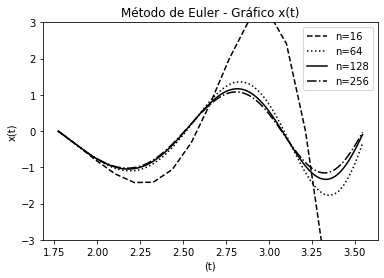
\includegraphics[scale=0.56]{eulerx_diferentesn}
\caption{Gráfico $x$ vs $t$ com diferentes valores de $n$.}
\label{eulerx_difn}
\end{figure}

\begin{figure}[H]
%\begin{figure}
\centering
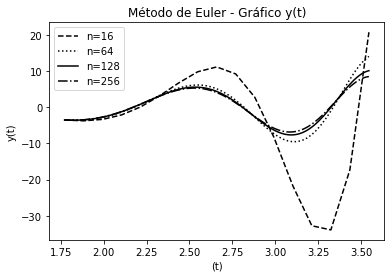
\includegraphics[scale=0.56]{eulery_diferentesn}
\caption{Gráfico $y$ vs $t$ com diferentes valores de $n$.}
\label{eulery_difn}
\end{figure}

Podemos observar que à medida que aumentamos o valor de $n$, ou seja, diminuímos o passo de integração $h$, as soluções se sobrepõem. A figura \ref{exatanumE} mostra o gráfico de $x(t)$ e $y(t)$ plotados juntos com relação a $t$ para $n=256$. 
\begin{figure}[H]
\centering
%\begin{figure}
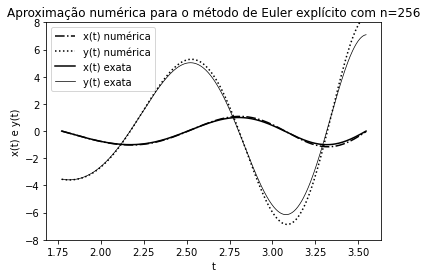
\includegraphics[scale=0.56]{exata_num_x_y}
\caption{Aproximação numérica para o método de Euler Explícito para $n=256$.}
\label{exatanumE}
\end{figure}

\begin{figure}[H]
%\begin{figure}
\centering
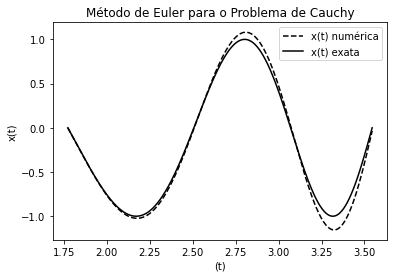
\includegraphics[scale=0.56]{eulerx_num_exata}
\caption{Gráfico $x$ vs $t$ da solução exata e numérica para $n=256$.}
\label{eulerx}
\end{figure}

\begin{figure}[H]
%\begin{figure}
\centering
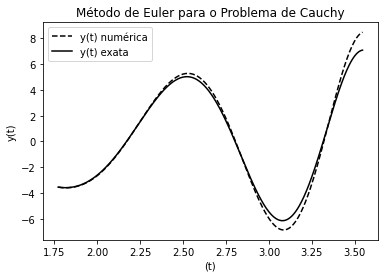
\includegraphics[scale=0.56]{eulery_num_exata}
\caption{Gráfico $y$ vs $t$ da solução exata e numérica para $n=256$.}
\label{eulery}
\end{figure}

Nos gráficos \ref{eulerx} e \ref{eulery} podemos ver que a solução numérica se aproxima de fato da solução exata do problema. Como $\mathbb{F}(t,\mathbb{Y})$ é continua e de \textit{Lipschitz} (ver \cite{numerical}), a função $\Phi(t,\mathbb{Y},h)$ também é contínua e de \textit{Lipschitz}. Portanto, para um instante de tempo fixado $t$, as soluções numéricas convergem para a solução exata à medida que o passo de integração vai para zero. Assim, o método de Euler é de fato convergente. Podemos verificar esse resultado na tabela \ref{tab1}.

\begin{table*}[htb]
  \centering
    \begin{tabular}{|r|r|r|r|r|}
      \hline
      $n$ &  $h$ &  $|e(t,h)|$ &  $|q=e(t,2h)/e(t,h)|$  &  ordem $p$ \\
      \hline\hline
	 4 & 0,25 & 2,225940517E+01 & &\\
	 8 & 1,250000000E-01 & 9,979693321E+00 & 2,2304699E+00 & 1,157348E+00\\
	 16 & 6,250000000E-02 & 3,037005329E+00 & 3,2860309E+00 & 1,716346E+00\\
	 32 & 3,125000000E-02 & 1,030780929E+00 & 2,9463150E+00 & 1,558912E+00\\
	 64 & 1,562500000E-02 & 4,111492263E-01 & 2,5070725E+00 & 1,326004E+00\\
	 128 & 7,812500000E-03 & 1,823123297E-01 & 2,2551916E+00 & 	1,173250E+00\\
	 256 & 3,906250000E-03 & 8,570527863E-02 & 2,1272007E+00 & 1,088956E+00\\
	 512 & 1,953125000E-03 & 4,153579562E-02 & 2,0634077E+00 & 1,045029E+00\\
	 1024 & 9,765625000E-04 & 2,044442139E-02 & 2,0316445E+00 & 1,022648E+00\\
	 2048 & 4,882812500E-04 & 1,014205784E-02 & 2,0158060E+00 & 1,011357E+00\\
	 4096 & 2,441406250E-04 & 5,051080183E-03 & 2,0078988E+00 & 1,005687E+00\\
	 8192 & 1,220703125E-04 & 2,520564089E-03 & 2,0039483E+00 & 
1,002845E+00\\
	16384 & 6,103515625E+04 & 1,259039441E-03 & 2,0019739E+00 & 1,001423E+00\\
      \hline
    \end{tabular}
    \caption{Tabela com erros de discretização global em $t$ fixo e suas razões para o Método de Euler Explícito.}
    \label{tab1}
\end{table*}

Para mostrar a convergência do método de Euler explícito, resolvemos a equação \ref{Explicito} para passos de integração progressivamente menores $h=\frac{(\sqrt{\pi}+1)- \sqrt{\pi}}{n}$, no instante $t = \sqrt{\pi}+1$ fixo, $n=2^{2+m}$ para $m=0,1,\ldots, 12$. A coluna $|e(t,h)|$ da tabela \ref{tab1} descreve o erro de discretização global a qual é dada por 
\begin{equation}
e(t_k,h) \doteq e_k \doteq \mathbb{Y}(t_k) - \mathbb{Y}_k
\end{equation} 
onde $\mathbb{Y}(t)$ é a solução exata \eqref{sol_exata} conhecida no instante $t=t_k$ e $\mathbb{Y}_k$ é o k-ésimo passo de integração do método numérico. Como o problema analisado é bidimensional, temos
\begin{equation}\label{errodiscr}
\begin{cases}
 e_x = x(t_k) - x_k \\ 
 e_y = y(t_k) - y_k \\
 |e(t,h)| = max ({|e_x|,|e_y}|)
\end{cases}
\end{equation} 

A quarta coluna da tabela \ref{tab1} mostra que à medida que o passo de integração é reduzido pela metade, o erro de discretização global também é. Isso ocorre a partir de um $h$ suficientemente pequeno. A última coluna nos mostra que o método de Euler explícito tem ordem $p =1$ para o instante $t = \sqrt{\pi} +1$. 

No entanto, podemos estimar a ordem de convergência do método numérico sem usarmos sua solução exata. A expansão \eqref{estimativaerro} fornece uma maneira para estimar a ordem em que o método numérico converge para a solução exata do problema, onde $\eta(t,h)$ são as soluções numéricas e $p$ a ordem teórica do método. 
\begin{equation}\label{estimativaerro}
e(t,\frac{h}{2}) \approx - \frac{\eta (t,h) - \eta(t,\frac{h}{2}) }{2^p -1}
\end{equation}

Para, de fato, estimarmos a ordem do método, precisamos calcular as aproximações numéricas para um $t$ fixado, $\eta(t,2h)$, $\eta(t,h)$ e $\eta(t,\frac{h}{2})$, , onde $h> 0$ é suficientemente pequeno. O próximo passo é calcular o valor absoluto do quociente entre as diferenças das aproximações, conforme
\begin{equation}\label{quociente}
\left| \frac{\eta(t,2h) - \eta(t,h)}{\eta(t,h) - \eta(t,h/2)} \right| \approx \left| \frac{e_{\tilde{p}}(t)(2^{\tilde{p}}-1)h^{\tilde{p}}}{e_{\tilde{p}}(t)(1-2^{-\tilde{p}})h^{\tilde{p}}} \right| = 2^{\tilde{p}}.
\end{equation}

O que resta agora é calcular o logaritmo de base 2 em \eqref{quociente} em que obteremos uma estimativa para $\tilde{p}$. Repetindo esse processo para passos sucessivamente menores, vamos obter uma sequência de estimativas $\tilde{p}_1, \tilde{p}_2, \cdots$ que convergirá para $\tilde{p}$. Repare que a ordem de convergência obtida numericamente $\tilde{p}$ pode não ser exatamente igual a $p$, ordem prevista para o método na teoria. No entanto, a sequência $\tilde{p}_1, \tilde{p}_2, \cdots$ obtida convergirá para $p$ à medida que $h$ se aproximar de zero. Outra questão a ser levantada é que utilizamos divisões sucessivas por $2$ para obtermos a sequência de passos de integração, mas nada impede que se possa utilizar qualquer outro número positivo $r$ onde teríamos $h/r, h/r^2, h/r^3, \cdot$. 

O código abaixo mostra o cálculo da estimativa de erro global para o método de Euler explícito.
\begin{lstlisting}
// Erro de discretizacao Euler - caso 2 quando usamos as aproximacoes no lugar da solucao exata
def ErroECaso2(t0, tfin, xin, yin, m, F):
    i=m //comeca com m=2
    qtdm=[]
    taberrog=[] //lista para o erro max entre erro_x e erro_y
    tabh=[]  //lista dos passos de integracao 
    n=2**m  
    tabq=[]  //lista da razao dos erros
    tabp=[] //lista das ordem numericas obtidas
    listax=[] //lista que guarda a ultima aproximacao calculada em x
    listay=[] //lista que guarda a ultima aproximacao calculada em y
    
    while i<=14:  //laco que calcula m =2,..14 
        h=(tfin-t0)/(2**i)
        qtdm.append(i)
        tabh.append(h)
        xE=Euler(t0, tfin, xin, yin, n, F)[1] //chama a funcao Euler e acessa a linha 1 (xsol)
        yE=Euler(t0, tfin, xin, yin, n, F)[2] //chama a funcao Euler e acessa a linha 2 (ysol)
        listax.append(xE[-1])
        listay.append(yE[-1])
        if i==3:
            errox=abs(-listax[-2] + listax[-1])
            erroy=abs(-listay[-2] + listay[-1])
            errog = max(errox,erroy)
            taberrog.append(errog)
        if i>3:
            errox=abs(-listax[-2] + listax[-1])
            erroy=abs(-listay[-2] + listay[-1])
            errog = max(errox,erroy)
            taberrog.append(errog)           
            q=abs((taberrog[-2])/(taberrog[-1]))
            tabq.append(q)
            p=math.log(q,2)
            tabp.append(p)
        i=i+1
        n=2**i
     
    return(qtdm,tabh,taberrog,tabq,tabp)

\end{lstlisting}


\begin{table*}[htb]
  \centering
    \begin{tabular}{|r|r|r|r|r|}
      \hline
      $n$ &  $h$ &  $|\eta(t,2h) - \eta(t,h)|$ &  $q$  &  ordem $p$ \\
       \hline \hline
 		4 & 0,25 & &  &\\
 		8 & 1,250000000E-01 & 12,27971185 & &\\
 		16 & 6,250000000E-02 & 6,942687992 & 1,7687259E+00 & 8,227105E-01\\
 		32 & 3,125000000E-02 & 2,0062244 & 3,4605740E+00 & 1,791011E+00\\
 		64 & 1,562500000E-02 & 0,619631703 & 3,2377691E+00 & 1,695000E+00\\
 		128 & 7,812500000E-03 & 0,228836897 & 2,7077439E+00 & 1,437091E+00\\
 		256 & 3,906250000E-03 & 0,096607051 & 2,3687391E+00 & 1,244119E+00\\
 		512 & 1,953125000E-03 & 0,044169483 & 2,1871900E+00 & 1,129079E+00\\
 		1024 & 9,765625000E-04 & 0,021091374 & 2,0941965E+00 & 1,066397E+00\\
 		2048 & 4,882812500E-04 & 0,010302364 & 2,0472365E+00 & 1,033678E+00\\
 		4096 & 2,441406250E-04 & 0,005090978 & 2,0236513E+00 & 1,016961E+00\\
 		8192 & 1,220703125E-04 & 0,002530516 & 2,0118337E+00 & 1,008511E+00\\
 		16384 & 6,103515625E+04 & 0,001261525 & 2,0059189E+00 & 1,004263E+00\\
       \hline
    \end{tabular}
    \caption{Estimativa numérica da ordem de convergência do Método de Euler Explícito no instante $t= \sqrt{\pi} +1$.}
    \label{tab2}
\end{table*}

A tabela \ref{tab2} foi gerada pelo código acima com $t= \sqrt{\pi} +1$ fixado, $n = 2^m$ para $m=2,\cdots, 14$.

Observe que a terceira coluna da tabela \ref{tab2} é o valor absoluto do quociente entre as diferenças das aproximações conforme equação \eqref{quociente}. E a quarta coluna é obtida quando calculamos o logaritmo de base $2$ da coluna anterior. Podemos ver que a sequência de estimativas $\tilde{p}_1, \tilde{p}_2, \tilde{p}_3, \cdots$ (coluna ordem $p$ - quarta coluna) à medida que o passo de integração $h$ diminui (se aproximando de zero), tende a ordem teórica do método, que neste caso é $1$.


\subsection{Método de Euler Aprimorado}
A discretização do problema para o método de Euler aprimorado de acordo com \eqref{def aprimorado} é dado por 
\begin{eqnarray}\label{Aprimorado}
\begin{cases}
\begin{pmatrix}  x_{k+1} \\ y_{k+1} \end{pmatrix}
 = \begin{pmatrix} x_k\\ y_k \end{pmatrix}
 +\dfrac{h}{2}.\\
 .\begin{pmatrix} f_1(t_k,x_k,y_k)+f_1(t_{k+1},x_k + hf_1(t_k,x_k,y_k),y_k) \\ f_2(t_k,x_k,y_k)+f_2(t_{k+1},x_k,y_k + hf_2(t_k,x_k,y_k))
 \end{pmatrix}
 \end{cases}
 \end{eqnarray}
 
A função a seguir foi implementada em Python para a obtenção das aproximações numéricas para este caso.
\begin{lstlisting}
def Eaprimorado(t0, tfin, xin, yin, n, F):
    i=1
    tsol=[t0]
    xsol=[xin]
    ysol=[yin]
    yn=np.array([xin, yin])
    dt=(tfin - t0)/n

    while i<=n:
        yn=yn +(dt/2)*(Phi(F,t0,yn,dt)[0] + Phi(F,t0,yn,dt)[1])
        tk=t0+dt
        xsol.append(yn[0])
        ysol.append(yn[1])
        tsol.append(tk)
        t0=tk
        xin=yn[0]
        yin=yn[1]
        i=i+1
    return(tsol,xsol,ysol)  
\end{lstlisting}

Os gráficos \ref{aprix_difn} e \ref{apriy_difn} mostram a solução para cada variável de estado $x(t)$ e $y(t)$ que compõem $\mathbb{Y}(t)$ variando os valores de $n$.
\begin{figure}[H]
\centering
%\begin{figure}
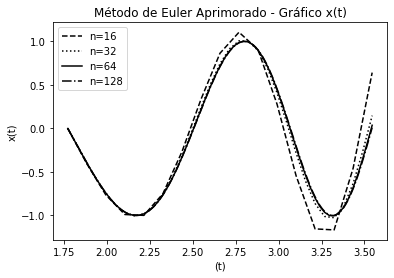
\includegraphics[scale=0.56]{aprix_diferentesn}
\caption{Gráfico $x$ vs $t$ com diferentes valores de $n$.}
\label{aprix_difn}
\end{figure}

\begin{figure}[H]
%\begin{figure}
\centering
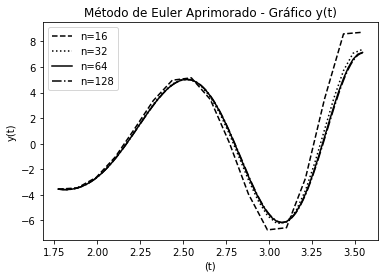
\includegraphics[scale=0.56]{apriy_diferentesn}
\caption{Gráfico $y$ vs $t$ com diferentes valores de $n$.}
\label{apriy_difn}
\end{figure}

Podemos observar que à medida que aumentamos o valor de $n$, ou seja, diminuímos o passo de integração $h$, as soluções se sobrepõem, da mesma forma que no método anterior. A figura \ref{exatanumA} mostra o gráfico de $x(t)$ e $y(t)$ plotados juntos com relação a $t$ para $n=32$. 
\begin{figure}[H]
%\begin{figure}
\centering
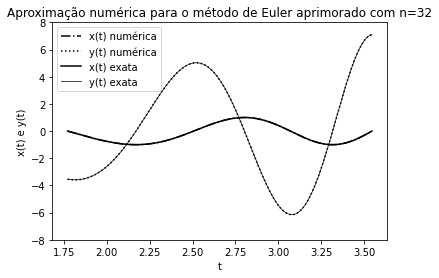
\includegraphics[scale=0.56]{exata_num_x_yA}
\caption{Aproximação numérica para o método de Euler Aprimorado para $n=32$.}
\label{exatanumA}
\end{figure}

\begin{figure}[H]
%\begin{figure}
\centering
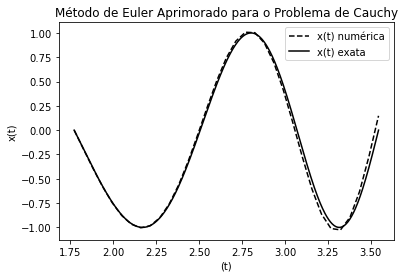
\includegraphics[scale=0.56]{aprix_num_exata}
\caption{Gráfico $x$ vs $t$ da solução exata e numérica para $n=32$.}
\label{aprix}
\end{figure}

\begin{figure}[H]
%\begin{figure}
\centering
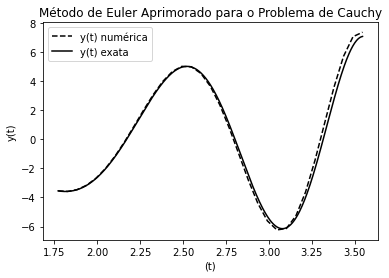
\includegraphics[scale=0.56]{apriy_num_exata}
\caption{Gráfico $y$ vs $t$ da solução exata e numérica para $n=32$.}
\label{apriy}
\end{figure}

Nos gráficos \ref{aprix} e \ref{apriy} podemos ver que a solução numérica também se aproxima de fato da solução exata do problema. A justificativa é a mesma que do método de Euler explícito. Como $\mathbb{F}(t,\mathbb{Y})$ é continua e de \textit{Lipschitz} (ver \cite{numerical}), a função $\Phi(t,\mathbb{Y},h)$ também é contínua e de \textit{Lipschitz}. Portanto, para um instante de tempo fixado $t$, as soluções numéricas convergem para a solução exata à medida que o passo de integração vai para zero. Assim, o método de Euler aprimorado é de fato convergente. Podemos verificar esse resultado na tabela \ref{tab3}.
\begin{table*}[htb]
  \centering
    \begin{tabular}{|r|r|r|r|r|}
      \hline
      $n$ &  $h$ &  $|e(t,h)|$ &  $|q=e(t,2h)/e(t,h)|$  &  ordem $p$ \\
       \hline \hline
       4 & 0,25 & 3,9724775E+00 & &\\
       8 & 1,250000000E-01 & 1,2000170E+00 & 3,3103511E+00 & 1,726984E+00\\
       16 & 6,250000000E-02 & 3,2084066E-01 & 3,7402272E+00	& 1,903126E+00\\
       32 & 3,125000000E-02 & 8,3541430E-02 & 3,8404976E+00 & 1,941293E+00\\
       64 & 1,562500000E-02 & 2,1324287E-02 & 3,9176658E+00 & 1,969994E+00\\
       128 & 7,812500000E-03 & 5,3856199E-03 & 3,9594861E+00 & 1,985313E+00\\
       256 & 3,906250000E-03 & 1,3531312E-03 & 3,9801164E+00 & 1,992811E+00\\
       512 & 1,953125000E-03 & 3,3911526E-04 & 3,9901809E+00 & 1,996454E+00\\
       1024 & 9,765625000E-04 & 8,4882265E-05 & 3,9951250E+00 & 1,998241E+00\\
       2048 & 4,882812500E-04 & 2,1233457E-05 & 3,9975716E+00 & 1,999124E+00\\
       4096 & 2,441406250E-04 & 5,3099729E-06 & 3,9987882E+00 & 1,999563E+00\\
       8192 & 1,220703125E-04 & 1,3276942E-06 & 3,9993947E+00 & 1,999782E+00\\
       16384 & 6,103515625E+04 & 3,3194866E-07 & 3,9996973E+00 & 1,999891E+00\\
       \hline
    \end{tabular}
    \caption{Tabela com erros de discretização global em $t$ fixo e suas razões para o Método de Euler Aprimorado.}
    \label{tab3}
\end{table*}

Para mostrar a convergência do método de Euler aprimorado, resolvemos a equação \eqref{Aprimorado} para passos de integração progressivamente menores $h=\frac{(\sqrt{\pi}+1)- \sqrt{\pi}}{n}$, no instante $t = \sqrt{\pi}+1$ fixo, $n=2^{2+m}$ para $m=0,1,\ldots, 12$ como no método de Euler explícito. A coluna $|e(t,h)|$ da tabela \ref{tab3} descreve o erro de discretização global do método aprimorado e foi calculado da mesma forma que em \eqref{errodiscr}

A quarta coluna da tabela \ref{tab2} mostra que à medida que o passo de integração é reduzido pela metade, o erro de discretização global também é. Isso ocorre a partir de um $h$ suficientemente pequeno. A última coluna nos mostra que o método de Euler aprimorado tem ordem $p =2$ para o instante $t = \sqrt{\pi} +1$. 

Da mesma forma que no método de Euler explícito, podemos estimar a ordem de convergência para o método de Euler aprimorado sem utilizarmos a solução exata do problema. Analogamente ao que foi construído anteriormente, obtemos a tabela \ref{tab4}.
\begin{table*}[htb]
  \centering
    \begin{tabular}{|r|r|r|r|r|}
      \hline
      $n$ &  $h$ &  $|\eta(t,2h) - \eta(t,h)|$ &  $q$  &  ordem $p$ \\
       \hline \hline
 		4 & 0,25 & & & \\
 		8 & 1,250000000E-01 & 9,2415351E-01 & &\\
 		16 & 6,250000000E-02 & 2,9305877E-01 & 	3,1534751E+00 & 1,656943E+00\\
 		32 & 3,125000000E-02 & 7,9099744E-02 & 3,7049269E+00 & 1,889445E+00\\
 		64 & 1,562500000E-02 & 2,0739048E-02 & 3,8140490E+00 & 1,931323E+00\\
 		128 & 7,812500000E-03 & 5,3128891E-03 & 3,9035348E+00 & 1,964781E+00\\
 		256 & 3,906250000E-03 & 1,3441629E-03 & 3,9525635E+00 & 1,982789E+00\\
 		512 & 1,953125000E-03 & 3,3800533E-04 & 3,9767506E+00 & 1,991590E+00\\
 		1024 & 9,765625000E-04 & 8,4744332E-05 & 3,9885302E+00 & 1,995857E+00\\
 		2048 & 4,882812500E-04 & 2,1216269E-05 & 3,9943088E+00 & 1,997946E+00\\
 		4096 & 2,441406250E-04 & 5,3078280E-06 & 3,9971660E+00 & 1,998977E+00\\
 		8192 & 1,220703125E-04 & 1,3274263E-06 & 3,9985860E+00 & 1,999490E+00\\
 		16384 & 6,103515625E+04 & 3,3191517E-07 & 3,9992938E+00 & 1,999745E+00\\
       \hline
    \end{tabular}
    \caption{Estimativa numérica da ordem de convergência do Método de Euler Aprimorado no instante $t=\sqrt{\pi} +1$.}
    \label{tab4}
\end{table*}

Observe que a terceira coluna da tabela \ref{tab4} é o valor absoluto do quociente entre as diferenças das aproximações calculadas pelo método de Euler aprimorado conforme equação \eqref{quociente}. A quarta coluna é obtida quando calculamos o logaritmo de base $2$ da coluna anterior. Além disso, podemos ver que a sequência de estimativas $\tilde{p}_1, \tilde{p}_2, \tilde{p}_3, \cdots$ (coluna ordem $p$ - quarta coluna) à medida que o passo de integração $h$ se aproxima de zero, tende a ordem teórica do método, que neste caso é $2$. Para a construção da tabela \ref{tab4} utilizamos o mesmo código que para o caso do método de Euler explícito, apenas chamamos a função \textit{Eaprimorado} para o cálculo das aproximações numéricas, como segue
\begin{lstlisting}
//Estimativa do erro de discretizacao sem solucao exata - caso2 tarefa-euler aprimorado
def ErroACaso2(t0, tfin, xin, yin, m, F):
    i=m
    qtdm=[]
    taberrog=[]
    tabh=[]
    n=2**m
    tabq=[]
    tabp=[]
    listax=[]
    listay=[]
    d = (2**2) -1 //euler aprimorado tem ordem p =2, denominador da Equacao 14
        
    while i<=14:
        h=(tfin-t0)/(2**i)
        qtdm.append(i)
        tabh.append(h)
        xE=Eaprimorado(t0, tfin, xin, yin, n, F)[1]
        yE=Eaprimorado(t0, tfin, xin, yin, n, F)[2]
        listax.append(xE[-1])
        listay.append(yE[-1])
        if i==3:
            errox=abs(-listax[-2] + listax[-1])
            erroy=abs(-listay[-2] + listay[-1])
            errog = max(errox,erroy)/d
            taberrog.append(errog)
        if i>3:
            errox=abs(-listax[-2] + listax[-1])
            erroy=abs(-listay[-2] + listay[-1])
            errog = max(errox,erroy)/d
            taberrog.append(errog)           
            q=abs((taberrog[-2])/(taberrog[-1]))
            tabq.append(q)
            p=math.log(q,2)
            tabp.append(p)
        i=i+1
        n=2**i
     
    return(qtdm,tabh,taberrog,tabq,tabp)
    \end{lstlisting}

\subsection{Método de Euler Implícito}
A discretização do problema \eqref{nossoPC} segundo o método dado por \eqref{def implicito} fornece 
\begin{eqnarray}\label{Implicito}
\begin{pmatrix}  x_{k+1} \\ y_{k+1} \end{pmatrix}
 = \begin{pmatrix} x_k \\ y_k \end{pmatrix}
 +h \begin{pmatrix} y_{k+1} \\ y_{k+1}/t_{k+1} - 4t_{k+1}^2x_{k+1}
 \end{pmatrix}
 \end{eqnarray}
 
Como já mencionado anteriormente, precisamos resolver uma equação algébrica em cada passo de integração para determinarmos a aproximação $x_{k+1},y_{k+1}$ das respectivas variáveis de estado de $\mathbb{Y}_{k+1}$. Para resolver esta equação algébrica é necessário algum método iterativo como por exemplo método do ponto fixo ou método de Newton. Contudo, vamos analisar a $\mathbb{F}(t, \mathbb{Y})$ reescrevendo-a da seguinte forma:
\begin{eqnarray}\label{Fimplicito}
 \mathbb{F}(t,\mathbb{Y})
  = \begin{pmatrix} y \\ y/t - 4t^2x \end{pmatrix} 
  = \begin{pmatrix} 0 \qquad 1 \\ - 4t^2 \qquad 1/t\end{pmatrix}
  \begin{pmatrix} x(t) \\ y(t) \end{pmatrix}
 \end{eqnarray}

De acordo com \eqref{nossoPC} e denotando 
\begin{eqnarray*}
A 
= \begin{pmatrix} 0 \qquad 1 \\ - 4t^2 \qquad 1/t\end{pmatrix}
\end{eqnarray*}
temos
\begin{eqnarray}\label{discrImpldefato}
\mathbb{Y}_{k+1} &=& \mathbb{Y}_k + h A \mathbb{Y}_{k+1} \nonumber \\
(\mathbb{I} - hA) \mathbb{Y}_{k+1} &=& \mathbb{Y}_k \nonumber \\
\mathbb{Y}_{k+1} &=& (\mathbb{I} - hA)^{-1} \mathbb{Y}_k
\end{eqnarray}
onde a equação \eqref{discrImpldefato} é de fato um passo de integração de Euler implícito, $\mathbb{I}$ a matriz identidade de ordem $2$ e $(\mathbb{I} - hA)^{-1}$ é a inversa de $\mathbb{I} - hA$. Esta manipulação algébrica foi possível devido a $\mathbb{F}(t, \mathbb{Y})$ ser linear. Caso contrário deveríamos utilizar um método iterativo para cada passo de integração no método implícito. 

Reescrevendo a equação \eqref{discrImpldefato} obtemos
\begin{eqnarray}\label{Fimplicito}
 \begin{pmatrix} x_{k+1} \\ y_{k+1} \end{pmatrix} 
  = \dfrac{1}{{(1-h/t_{k+1})} + 4h^2t_{k+1}^2} \begin{pmatrix} (1-h/t_{k+1})x_k + hy_k \\ - 4t_{k+1}^2hx_k + y_k \end{pmatrix}
   \end{eqnarray}

Em Python, a função foi implementada conforme
\begin{lstlisting}
def Eimplicito(t0, tfin, xin, yin, n, F):
    i=1
    tsol=[t0]
    xsol=[xin]
    ysol=[yin]
    yn=np.array([xin, yin])
    dt=(tfin - t0)/n
    
    while i<=n:
        tk=t0 + dt
        c=1/((1-(dt/tk)) + 4*((dt)**2)*((tk)**2)) 
        xk= ((1-(dt/tk))*xin +dt*yin)*c
        yk=((-4*(tk**2)*dt*xin) +yin)*c 
        xsol.append(xk)
        ysol.append(yk)
        tsol.append(tk)
        t0=tk
        xin=xk
        yin=yk
        i=i+1
    return(tsol,xsol,ysol)
\end{lstlisting} 

Os gráficos \ref{implx_difn} e \ref{imply_difn} mostram a solução para cada variável de estado $x(t)$ e $y(t)$ que compõem $\mathbb{Y}(t)$ variando os valores de $n$.
\begin{figure}[H]
%\begin{figure}
\centering
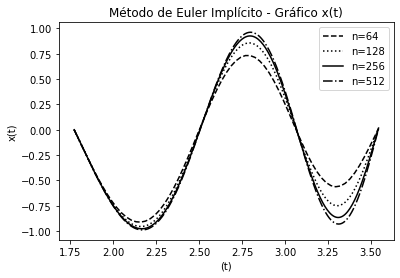
\includegraphics[scale=0.56]{implx_diferentesn}
\caption{Gráfico $x$ vs $t$ com diferentes valores de $n$.}
\label{implx_difn}
\end{figure}

\begin{figure}[H]
%\begin{figure}
\centering
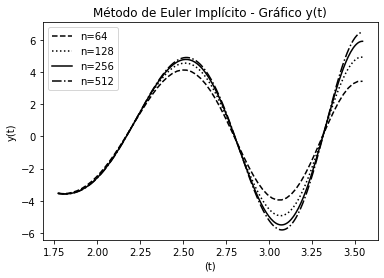
\includegraphics[scale=0.56]{imply_diferentesn}
\caption{Gráfico $y$ vs $t$ com diferentes valores de $n$.}
\label{imply_difn}
\end{figure}

Podemos observar que à medida que aumentamos o valor de $n$, ou seja, diminuímos o passo de integração $h$, as soluções se sobrepõem. A figura \ref{exatanumI} mostra o gráfico de $x(t)$ e $y(t)$ plotados juntos com relação a $t$ para $n=256$. 
\begin{figure}[H]
%\begin{figure}
\centering
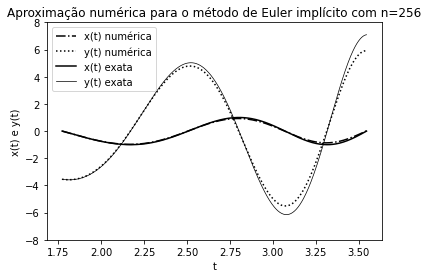
\includegraphics[scale=0.56]{exata_num_x_yI}
\caption{Aproximação numérica para o método de Euler Implícito para $n=256$.}
\label{exatanumI}
\end{figure}

\begin{figure}[H]
%\begin{figure}
\centering
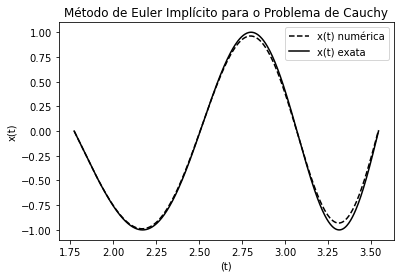
\includegraphics[scale=0.56]{implx_num_exata}
\caption{Gráfico $x$ vs $t$ da solução exata e numérica para $n=256$.}
\label{implx}
\end{figure}

\begin{figure}[H]
%\begin{figure}
\centering
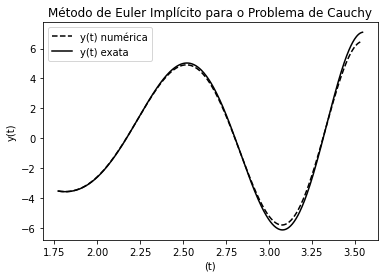
\includegraphics[scale=0.56]{imply_num_exata}
\caption{Gráfico $y$ vs $t$ da solução exata e numérica para $n=256$.}
\label{imply}
\end{figure}

Nos gráficos \ref{implx} e \ref{imply} podemos ver que a solução numérica se aproxima de fato da solução exata do problema. Portanto, para um instante de tempo fixado $t$, as soluções numéricas convergem para a solução exata à medida que o passo de integração vai para zero. Assim, o método de Euler implícito é de fato convergente. Podemos verificar esse resultado na tabela \ref{tab5}. 
\begin{table*}[!htb]
  \centering
    \begin{tabular}{|r|r|r|r|r|}
      \hline
      $n$ &  $h$ &  $|e(t,h)|$ &  $|q=e(t,2h)/e(t,h)|$  &  ordem $p$ \\
       \hline \hline
       4 & 0,25 & 9,2495030E-01 & &\\
       8 & 1,250000000E-01 & 7,2657266E-01 & 1,2730321E+00 & 0,348268772\\
       16 & 6,250000000E-02 & 4,8532384E-01 & 1,4970883E+00 & 0,582159349\\
       32 & 3,125000000E-02 & 3,7874574E-01 & 1,2813975E+00 & 0,357718078\\
       64 & 1,562500000E-02 & 2,4836030E-01 & 1,5249850E+00 & 0,60879506\\
       128 & 7,812500000E-03 & 1,4163380E-01 & 1,7535384E+00 & 0,810268989\\
       256 & 3,906250000E-03 & 7,5536895E-02 & 1,8750281E+00 & 0,906912207\\
       512 & 1,953125000E-03 & 3,8993779E-02 & 1,9371525E+00 & 0,953937507\\
       1024 & 9,765625000E-04 & 1,9808922E-02 & 1,9684957E+00 & 0,977093594\\
       2048 & 4,882812500E-04 & 9,9831834E-03 & 1,9842290E+00 & 0,988578559\\
       4096 & 2,441406250E-04 & 5,0113616E-03 & 1,9921100E+00 & 0,994297288\\
       8192 & 1,220703125E-04 & 2,5106344E-03 & 1,9960539E+00 & 0,997150655\\
       16384 & 6,103515625E+04 & 1,2565570E-03 & 1,9980267E+00 & 0,998575831\\
       \hline
    \end{tabular}
    \caption{Tabela com erros de discretização global em $t$ fixo e suas razões para o Método de Euler Implícito.}
    \label{tab5}
\end{table*}

Para mostrar a convergência do método, resolvemos o problema para passos de integração progressivamente menores $h=\frac{(\sqrt{\pi}+1)- \sqrt{\pi}}{n}$, no instante $t = \sqrt{\pi}+1$ fixo, $n=2^{2+m}$ para $m=0,1,\ldots, 12$. A coluna $|e(t,h)|$ da tabela \ref{tab5} descreve o erro de discretização global do método e foi calculado da mesma forma que em \eqref{errodiscr}

A quarta coluna da tabela \ref{tab5} mostra que à medida que o passo de integração é reduzido pela metade, o erro de discretização global também é. Isso ocorre a partir de um $h$ suficientemente pequeno. A última coluna nos mostra que o método de Euler implícito tem ordem $p =1$ para o instante $t = \sqrt{\pi} +1$.  

Da mesma forma que nos métodos anteriores, podemos estimar a ordem de convergência para o método de Euler aprimorado sem utilizarmos a solução exata do problema. Analogamente ao que já foi apresentado, obtemos a tabela \ref{tab6}.
\begin{table*}[!htb]
  \centering
    \begin{tabular}{|r|r|r|r|r|}
      \hline
      $n$ &  $h$ &  $|\eta(t,2h) - \eta(t,h)|$ &  $q$  &  ordem $p$ \\
       \hline \hline
 		4 & 0,25 & & & \\
 		8 & 1,250000000E-01 & 1,9837764E-01 & &\\
 		16 & 6,250000000E-02 & 2,4124882E-01 & 8,2229477E-01 & -0,282272441 \\
 		32 & 3,125000000E-02 & 2,0407203E-01 & 1,1821749E+00 & 0,241443447\\
 		64 & 1,562500000E-02 & 1,3068719E-01 & 1,5615305E+00 & 0,642960732\\
 		128 & 7,812500000E-03 & 1,0672650E-01 & 1,2245055E+00 & 0,292199245\\
 		256 & 3,906250000E-03 & 6,6096905E-02 & 1,6146974E+00 & 0,691263832\\
 		512 & 1,953125000E-03 & 3,6543116E-02 & 1,8087375E+00 & 0,854983054\\
 		1024 & 9,765625000E-04 & 1,9184857E-02 & 1,9047896E+00 & 0,929631663\\
 		2048 & 4,882812500E-04 & 9,8257389E-03 & 1,9525104E+00 & 0,965330199\\
 		4096 & 2,441406250E-04 & 4,9718218E-03 & 1,9762854E+00 & 0,982791318\\
 		8192 & 1,220703125E-04 & 2,5007271E-03 & 1,9881504E+00 & 0,991426929\\
 		16384 & 6,103515625E+04 & 1,2540774E-03 & 1,9940772E+00 &	0,995721247\\
 		\hline
    \end{tabular}
    \caption{Estimativa numérica da ordem de convergência do Método de Euler Implícito no instante $t=\sqrt{\pi} +1$.}
    \label{tab6}
\end{table*}

Observe que a terceira coluna da tabela \ref{tab6} é o valor absoluto do quociente entre as diferenças das aproximações calculadas pelo método de Euler implícito conforme equação \eqref{quociente}. A quarta coluna é obtida quando calculamos o logaritmo de base $2$ da coluna anterior. Além disso, podemos ver que a sequência de estimativas $\tilde{p}_1, \tilde{p}_2, \tilde{p}_3, \cdots$ (coluna ordem $p$ - quarta coluna) à medida que o passo de integração $h$ se aproxima de zero, tende a ordem teórica do método, que neste caso é $1$. 

Para a construção da tabela \ref{tab6} utilizamos o mesmo código que para os dois casos anteriores, apenas chamamos a função \textit{Eimplicito} para o cálculo das aproximações numéricas. 

\begin{lstlisting}
// estimativa do erro de discretizacao para euler implicito
def ErroICaso2(t0, tfin, xin, yin, m, F):
   //
   // igual aos codigos anteriores para estimativa de erro     
    while i<=14:
       //
       //parte igual a do euler explicito
       //
        xE=Eimplicito(t0, tfin, xin, yin, n, F)[1]
        yE=Eimplicito(t0, tfin, xin, yin, n, F)[2]
        listax.append(xE[-1])
        listay.append(yE[-1])
        if i==3:
        //
        //igual a euler explicito 
     	//
\end{lstlisting}

%%%%%%%%%%%%%%%%%%%%%%
%%%%%%%%%%%%%%%%%%%%%%
\section{Conclusão}

Este trabalho analisou métodos de passo simples de Euler explícito, aprimorado e implícito através de um problema de Cauchy. Verificamos que os métodos são convergentes aproximando a solução numérica da solução exata do problema. Além disso, apresentamos os principais algoritmos implementados em Python para a resolução do problema para os diferentes métodos.   

%\newpage
\bibliographystyle{plain}
\bibliography{biblio}
\end{document}
